\section{Observations} 
\label{891_1:sec:obs}

Observations of NGC 891 were obtained over two runs in November and
December of 2014. Data were collected with the \GP IFU, coupled to the
WIYN Bench Spectrograph.

\begin{deluxetable}{lcc}
\tablewidth{0pt}
\tablecaption{Spectrograph Setup}
\tablehead{
  \colhead{Parameter} &
  \colhead{Value} &
  \colhead{Units}
}
\startdata
Grating Name & 400@4.2 & -\\
Order & 1 & -\\
Grating Angle & 21.53 & deg.\\
Camera-Collimator Angle & 30.00 & deg.\\
Anamorphic factor & 0.941 & -\\
$\lambda_\mathrm{min}\tablenotemark{a}$ & 3372 & \AA\\
$\lambda_\mathrm{max}\tablenotemark{a}$ & 7640 & \AA\\
Dispersion at \val{5500}{\AA}\tablenotemark{b} & 2.079 & \AA/pix
\enddata
\label{tab:spec}
\tablenotetext{a}{Formal wavelength range; values
  used for analysis are between 3850 and 6650\AA\ as described in the
  text.} 
\tablenotetext{b}{For 2$\times$ binning in the spectral dimension.}
\end{deluxetable}

\begin{deluxetable}{ccllc}
\tablewidth{0pt}
\tablecaption{Program Targets}
\tablehead{
  \colhead{Name} &
  \colhead{Type} &
  \colhead{$\alpha$} &
  \colhead{$\delta$} &
  \colhead{epoch}
}
\startdata
NGC 891 P1 & object & 02:22:29.7 & +42:19:17.2 & 2000\\
NGC 891 P2 & object & 02:22:32.5 & +42:20:26.0 & 2000\\
NGC 891 P3 & object & 02:22:37.6 & +42:22:38.3 & 2000\\
NGC 891 P4 & object & 02:22:30.1 & +42:21:33.7 & 2000\\
NGC 891 P5 & object & 02:22:26.8 & +42:18:07.9 & 2000\\
NGC 891 P6 & object & 02:22:40.4 & +42:23:57.0 & 2000\\
BD 284211 & flux standard & 21:48:57.1 & +28:37:48.0 & 1950\\
Feige 110 & flux standard & 23:17:23.5 & -05:26:22.0 & 1950
\enddata
\label{tab:targets}
\end{deluxetable}

\subsection{Spectrograph Configuration}

For both runs the spectrograph was configured identically to cover as
far blueward of the 4000\AA-break as practically possible while
reaching as far red as H$\alpha$.  The scientific motivation for this
large baseline was to capture Ca H\&K (3934,3968 \AA; this also
includes H$\epsilon$), the G-band ($\sim$4304 \AA), MgI
($\sim$5175 \AA), and the upper Balmer series (at least up to
H$\delta$), all important diagnostics for stellar populations; to
provide a measure of the continuum slope to determine reddening
independent of stellar age; and to have additional checks on the
extinction as derived from the ratio of \Ha/\HB emission line fluxes
(i.e., the Balmer decrement).

Achieving such a broad wavelength range that extends to the blue with
the Bench Spectrograph is challenging. This is due primarily to the
decreasing transmission of the spectrograph optics and fibers and
decreasing CCD quantum efficiency below 4500 \AA. In addition, as a
single beam spectrograph with all-refractive optics, the ability to
focus over a broad wavelength range extending to the blue is limited,
despite the ability to tilt the detector to compensate for chromatics.
Lastly, the grating suite is not optimal. Two 600 l/mm gratings are
just able to capture from, e.g., 3800-6650 \AA, which would enable us
to just capture the Fraunhofer L-band and H$\eta$ features between
3810-3840 \AA\ in the blue, and the redder [NII] line at 6584 \AA\ in the
red. Unfortunately these gratings are blazed too far to the red to
provide adequate overall efficiency in the blue.

We used engineering time to test alternative spectrograph
configurations with improved performance in the blue.  As we show in
Appendix \ref{891_1:sec:grating} compared to the best alternative 600 l/mm
grating, the very low (blue) blaze of the 400@4.2 grating yields
better performance below 4500 \AA\ (a factor of 2 increase in total
system efficiency at 4000 \AA), and broader wavelength coverage, albeit
with a 37\% lower spectral resolution. Because of the importance of
the blue spectral region, we chose this grating for our
observations. The detailed configuration provided in Table
\ref{tab:spec}.

While our spectrograph configuration covers between 3372 and 7640 \AA\
(the blaze wavelength is 3496 \AA) on the detector, in practice the
useful blue limit of the data is roughly \val{3850}{\AA} due to the
sharp decline in system efficiency. This captures H$\zeta$ and
sufficient pseudo-continuum to define a break amplitude \citep[e.g.,
$D_n4000$;][]{Balogh99}. The Fraunhofer L-band and H$\eta$ features
between 3810-3840 \AA\ are clearly visible in the highest
signal-to-noise data, while the strong FeI blends in the 3700-3750
\AA\ region and the Balmer break (3646 \AA) are not detected.  At the
red end of our wavelength range defocus becomes a serious problem and
fiber traces begin to blend significantly. This defocus, and the rise
of strong atmospheric OH features, sets the usable red limit to
\val{6650}{\AA}; this still captures \Ha and [NII] lines.

\subsection{Targeting}
\label{891_1:sec:targeting}

\begin{deluxetable}{cccll}
\tablewidth{0pt}
\tablecaption{Summary of Observations}
\tablehead{ 
  \colhead{Pointing} & 
  \colhead{Date} & 
  \colhead{$r$} & 
  \multicolumn{2}{c}{Integration (min)}\\
  \colhead{} &
  \colhead{(UT)} &
  \colhead{(kpc)} &
  \colhead{Nightly} &
  \colhead{Total}
}
\startdata 
1 & 2014 Nov 20 & 4.4      & 210 & $\cdots$ \\
  & 2014 Nov 21 & $\cdots$ &  60 & 270 \\
2 & 2014 Nov 21 & 0.8      & 210 & $\cdots$ \\
  & 2014 Nov 22 & $\cdots$ &  60 & 270 \\
3 & 2014 Nov 23 & $-6.4$   & 330 & 330 \\
4 & 2014 Nov 24 & $-2.3$   & 270 & 270 \\
5 & 2014 Dec 20 & 8.1      & 270 & $\cdots$ \\
  & 2014 Dec 22 & $\cdots$ & 270 & 540 \\
6 & 2014 Dec 21 & $-10.0$  & 240 &  $\cdots$ \\
  & 2014 Dec 23 & $\cdots$ & 120 & $\cdots$ \\
  & 2014 Dec 24 & $\cdots$ & 180 & 540
\enddata
\label{tab:obslog}
\end{deluxetable}

We observed NGC 891 with 6 pointings of \GP spanning a radial range
between \val{\asim 0.8}{kpc} $< \left|r\right| <$ \val{\asim 10}{kpc},
as given in Table \ref{tab:targets}. We chose pointings covering both
approaching and receding sides of the galaxy because of the known
asymmetry in star-formation and orientation of what appears to be a
two-armed spiral \citep{Xilouris99,Schechtman-Rook12}. In particular,
the approaching side appears to have significantly more H$\alpha$
emission and visible star-formation \citep{Rand90,Howk00,Kamphuis07a},
with the spiral arm closer along the line of sight. \cite{Kamphuis07b}
claim the star-formation asymmetry based on H$\alpha$ emission is
over-estimated due to differential attenuation effects, but
nonetheless the 24$\mu$m emission indicates at least a 30\% difference
in current star-formation on the two projected halves of the
galaxy. Furthermore, The HI distribution is also asymmetric, with an
extension to larger radii at lower column-density on the receding side
\citep{Swaters97,Oosterloo07}, although a similar asymmetry has not
been detected in CO \citep{Scoville93} possibly because of lack of
depth or coverage. Throughout this paper we use sign convention for
radius to be negative corresponding to the approaching (NE) side and
positive corresponding to the receding (SW) side.

To probe the known radial variations in disk components of NGC 891 on
both sides of the disk while continuously sampling in $|r|$, pointings
are staggered across the two sides of the galaxy. The inner two \GP
pointings (P2 and P4), on opposite sides of the center, sample within
the {\it inner} truncation of the thin and super-thin disk components,
as reckoned by \citet{Schechtman-Rook13}; this region is dominated by
a thickened, vertically exponential layer with a similar scale-height
to the thick-disk seen in the outer radial regions. This inner region
displays bar-like x-shaped isophotes, and the extended luminosity is
not that of a classical bulge. P1, P3, and P5 sample the region of the
super-thin disk. The outermost \GP pointing, P6, probes the region
beyond which there appears to be a super-thin disk as reckoned by NIR
broad-band photometry \citep{Schechtman-Rook12}, i.e., beyond the
outer truncation of the super-thin disk.

\begin{figure}
  \centering
  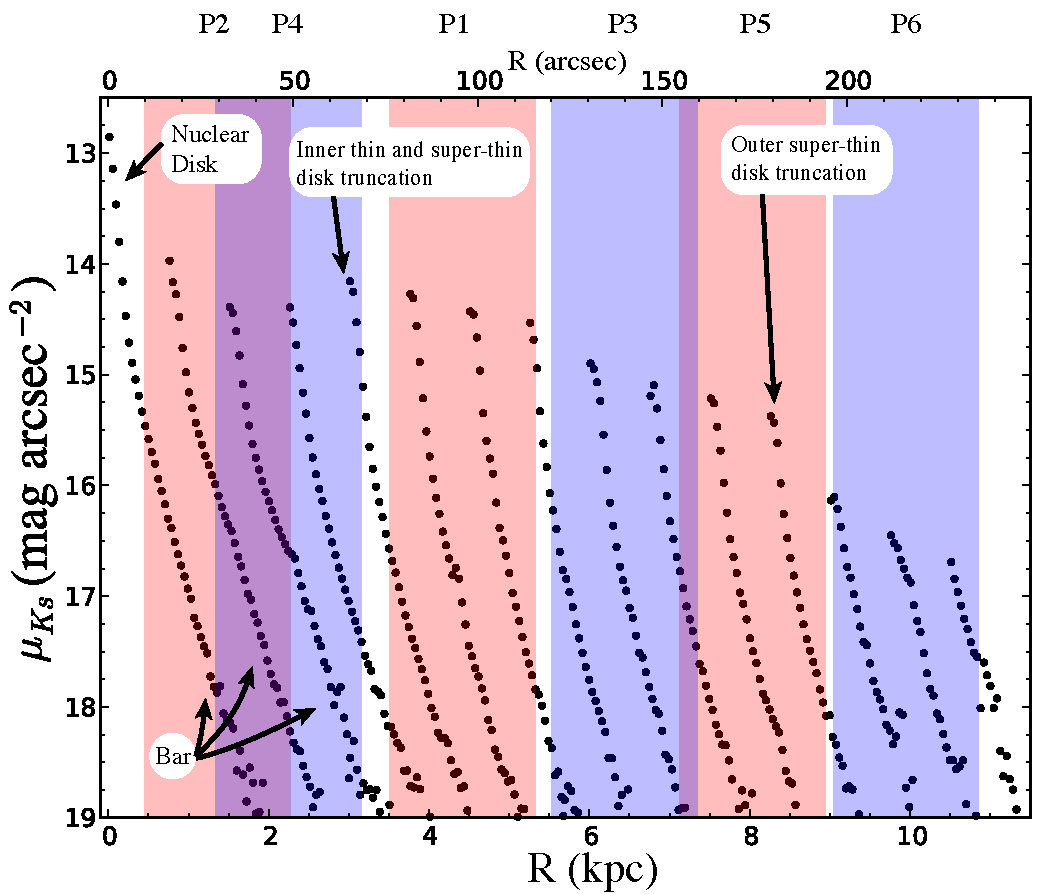
\includegraphics[width=\columnwidth]{891_1/figs/ASR_pointings.pdf}
  \caption{\label{fig:ASR_comp}\fixspacing Comparison of our \GP
    pointings to attenuation-corrected K-band light profiles measured
    by \citet{Schechtman-Rook13}. Important morphological features
    from that work are labeled with arrows. Shaded regions show the
    radial extent of each \GP pointing. Positive values of radius
    (receding) are red and negative radius values (approaching) are
    blue. The innermost \GP pointings were chosen be within the inner
    disc truncation visible in the density profiles.}
\end{figure}

Figure \ref{fig:ASR_comp} shows our \GP pointings related to the
results of \citet{Schechtman-Rook13}, Figure \ref{fig:pointings}
contains a pointing map, and a summary of observations can be found in
Table \ref{tab:obslog}. Ideally we would have observed both the
southern vertical half of the extended disk as well as the northern
vertical half. However, our pointings cover the full inner
\val{0.5}{kpc} of the disk mid-plane in height and we anticipate
vertical asymmetries between the two half of the galaxy at larger
heights are modest compared to radial variations on the approaching
and receding sides.

\begin{figure*}
  \centering
  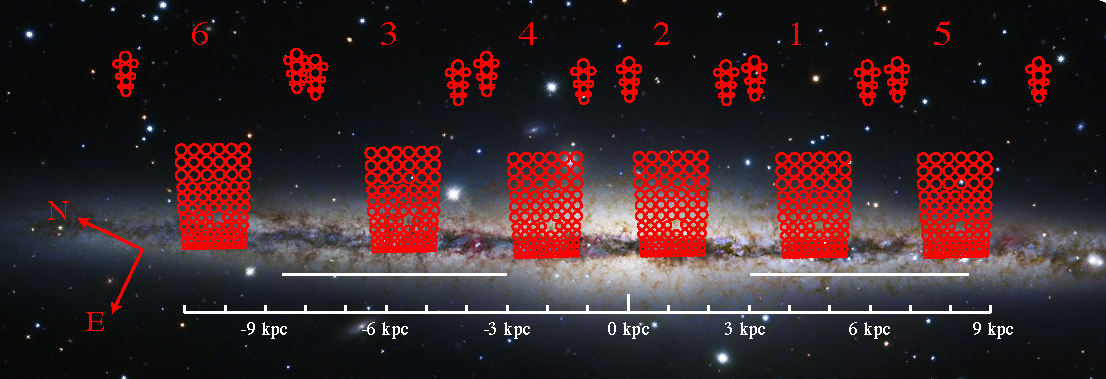
\includegraphics[width=\textwidth]{891_1/figs/NGC_891_better_pointings.pdf}
  \caption{\label{fig:pointings}\fixspacing NGC 891 \GP pointings
    (Table \ref{tab:targets}) overlaid on combined Subaru (V
    band)/West Mountain Observatory (R,G,B) image. The horizontal
    white lines denote the extent of the super-thin disk reported by
    \citet{Schechtman-Rook13}. \emph{Image credit:} Robert Gendler,
    NAOJ, HST/NASA, BYU (Michael Joner, David Laney). In this
    orientation the approaching side is to the left.}
\end{figure*}

All individual exposures for NGC 891 were 30 min in duration. This
exposure time was chosen so that the dominant random error in the
measured counts is caused by photon shot-noise from the sky and galaxy
flux, and not detector read-noise. To further beat down the read-noise
all exposures were binned 2x2 before readout, which still allowed for
adequate sampling of the smallest fibers (\val{\asim 2}{pixels} full
width at half maximum in both the spectral and spatial
dimensions). The total integration time for each pointing varies with
radius and are based on the requirement of the MaNGA survey
\citep{Bundy15} to measure absorption line indices sensitive to age
and metallicity. This S/N limit is roughly 50 per resolution
element. In practice the complex structure of NGC 891 lowers this
limit, but, as shown in \S\ref{891_1:sec:snr_threshold}, a S/N of 50 is
larger than required for full-spectrum SSP fitting. Some extra time
left at the end of our program was used to increase the observation
time (and therefore S/N) of the outermost pointings (5 and 6) where
the signal was expected to be lowest.

For all \GP observations the PA offset was 295.79$^{\circ}$ (East of
North), which is slightly offset from perfectly perpendicular to the
disk of NGC 891. This offset allows each fiber to occupy a unique
location in $z$, but is small enough to not affect the differential
light-gathering power unique to \GP.

In all tables and future discussion in this paper and papers in this
series we define negative radii to be the NE side of NGC 891. This is
consistent with \citet{Oosterloo07}, who's HI data show that negative
radii correspond to the approaching side of the disk.

\subsection{Calibration Data}
\label{891_1:sec:cal_data}

In addition to on-sky galaxy exposures we took bias, dark, dome-flat,
CuAr arc lamp, and standard star exposures for use during data
reduction. Standard star and other calibration exposures were short
enough ($<\val{2}{min}$) that dark current was not a significant
source of noise for these frames. Unfortunately, for the longer
exposures the elevated dark current of the Lincoln Labs STA1 (SN 5644)
CCD currently used on the Bench requires accurate dark-frame
subtraction for any work approaching sky-limited surface-brightness
levels.  Dark frames were 30 minutes long (i.e., the length of a
single object exposure) and taken during the day, between nightly
observations.

Due to tight scheduling at WIYN we were only able to observe dome
flats and arc lamps at the beginning of each night. Comparisons
of these frames across nights (and even from month-to-month) show that
the Bench Spectrograph is stable following 30 minutes from a dewar
fill. Once-a-night calibration frames are adequate for accurate data
reduction so long as the spectrograph configuration is not changed.

The presence of multiple fiber sizes in \GP required modifications to
the standard calibration procedure for dome flats and standard
stars. In particular, two sets of dome flats at different exposures
are needed: one set with a short (\val{1}{sec.}) exposure time to
avoid saturating the largest fibers, and one set with a longer
(\val{4}{sec.}) exposure time to get enough signal in the smallest
fibers. These two sets are combined during data reduction as described
in \S\ref{891_1:sec:flats}.

Once during each of the observing runs a set of blank sky observations
was recorded during twilight (i.e., sky flats). Due to the challenging
nature of flat observations described above these flats were not
deemed suitable for use during data reduction, but we are optimistic
that further investigation and experimentation with sky flats can
yield success for future \GP programs.

Nightly observations were made of two standard stars taken from the
IDS Photometric Standards catalog, listed in Table \ref{tab:targets},
and were made \asim 2 times per star per night. The \GP fibers have a
broad range of sizes, which, at the smallest, are insufficient to
capture the entire PSF. Further, because of atmospheric refraction,
the amount of light lost in the smaller fibers varies with wavelength.
%% See Figure
%% \ref{fig:DAR} for an example of this effect and section
%% \ref{891_1:sec:flux_cal} for implications of this decision on our reduced
%% data.  
While scanning the stars across the fibers at the parallactic
angle would eliminate wavelength-dependent effects, the available
telescope software was not up to this task. Consequently, we chose to
use only the largest (5.62 arcsec diameter) fibers for standard star
observations. Each set of standard star observations used 2-4 fibers
so that over the course of the entire observing program all of the
5.62'' had been used to observe the standard stars. Application of
these observations to flux calibrating the NGC 891 observations is
described in \S\ref{891_1:sec:flux_cal}.

%% {\bf [TO DO: Explain how many different, large fibers were calibrated with
%%     standard-star exposures. See comments and give better description of
%%     Figure \ref{fig:DAR} if we decide to keep it or a modified version.]}

%% \begin{figure}
%%   \centering
%%   \includegraphics[width=\columnwidth]{figs/DAR.png}
%%   \caption{\label{fig:DAR} Standard star observed through multiple fiber
%%     sizes. For this observation \GP was dragged across the standard star to
%%     sample all 5 fiber sizes. The effects of DAR are clearly visible as the
%%     supression of the blue end of the spectrum in the 3” and 2” fibers (and a
%%     little bit in the 4” fibers). {\bf [TO DO for this figure: Decide if we
%%         want to include it. It might be better to show the ratio of these
%%         normalized spectra. Also wondering if we really want to get into these
%%         scans. I don't know if they were made at the same off-paralactic
%%         angle. Do you have this information? The reason to show a figure like
%%         this would be to demonstrate that our flux cal with the large fibers
%%         is likely not missing light in a wavelength differential sense. BIGGER
%%         LABELS]}}
%% \end{figure}

%% We attempted to reduce the effects of DAR in smaller fibers by dragging
%% the standard star across the IFU directly along the altitude axis, but found
%% that this did not provide substantial enough mitigation to warrent the added
%% time cost of such a procedure (\val{\sim 30}{min}).

%% Here we summarize the observing runs (number of nights, conditions),
%% spectrograph setup, objects, and positions per object. For the
%% spectrograph setup give the grating(s), grating angle ($\alpha$),
%% camera-collimator angle, central wavelength, dispersion, spectral
%% coverage and range of spectral resolution over the range of fibers
%% sizes.

%% Describe salient features of observations, such as calibration.  It is
%% worth mentioning need for dark frames.  Standard-star observations and
%% lessons learned from trying to drift vs using large fibers is
%% important to describe. The key point to mention is that we use the
%% largest fibers to eliminated DAR effects from the flux calibration. Do
%% we worry about telluric absorption over our observed range of
%% wavelengths, and if not what is the impact (what are the relative
%% strengths and wavelengths of the strongest features)? If we do worry
%% about telluric correction, how do we handle the varying spectral
%% resolution with fiber size?

%% Other calibration data, e.g., twilight flats?
